\section{Experiments}
\label{sec:experiments}

\subsection{Data Sets}

We evaluated our implementations of various algorithms on 3 diverse datasets. The feature sets include real numbers, intergers and categorical values. The datasets are randomly split into training sets $80\%$ and
testing sets $20\%$. For multi-class data sets we do one-vs-all (OVA)
classifiers. For approximations that has reasonable run time, we will perform
cross-validation to select parameters for prior, which may have profound
impact on the result as suggested by~\cite{Asuncion2009smoothing}. Details of each dataset can found in Table~\ref{tb:datasets}.

\begin{table}
\begin{center}
\begin{tabular}{| c | c |  c | c | c |}
  \hline
  Datasets & \# training instances & \# test instances & \# features & class-wise split\\
  \hline
  Yeast & 1500 & 917 & 103 & (14 classes) \\
  \hline
  Spambase & 3680 & 921 & 57 & 39\% vs. 61\% \\
  \hline
  Heart Diseases & 216 & 54 & 13 & 44\% vs. 56\% \\
  \hline
\end{tabular}
\end{center}

\caption{Datasets information}
\label{tb:datasets}
\end{table}

\subsection{Results and Discussions}

Fig.~\ref{fig:results} shows the comparison of classification accuracy
(Fig.~\ref{fig:results} top) and run-time (bottom) of the four approximation
methods we consider. We find that sampling method outperforms all variational
inferences on all three datasets by substantial margins ($6-7\%$). This is
likely because all three variational methods make the Gaussian assumption of
the posterior, whereas the posterior of sampling is not limited to any
parametric form. 

Among the three variational approaches, Jaakkola {\it et al.} performs the
best. This does not necessarily imply that the variational lower bound in
Jaakkola {\it et al.} is tigher than the others. In fact, Jaakkola {\it et
al.} outperforms the other variational methods due to technical reasons: it
takes about 2 iterations for Jaakkola {\it et al.} to converge fully without
any tuning, which is not the case in Laplace and Delta method. In the latter
two approaches, the step size could effect the convergence of the gradient
descent type of algorithms. Furthermore, Delta method involves a matrix
inversion at each update and is computationally intensive. Thus it is very
possible that the resulted posterior has not fully converged in the prescribed
number of iterations. The poor results from Delta method is a testament to the
fragile nature of these approximation algorithms.

Due to these technical issues, we focus on the results of Yeast dataset. The
dataset has been previously studied by Wang {\it et al.}~\cite{Wang13}; they
reported similar classification accuracies which we tabulate in
Table~\ref{tab:compare_wang}. The difference is within $0.5\%$ for all three
methods, suggesting that these variational algorithms have properly converged.
These are strong evidences that our results are the optimal or near-optimal
performance from these variational methods. Interestingly, they all
``max-out'' at around $80\%$ classification accuracy, possibly due to the
Gaussian posterior assumption shared among these methods. On the other hand,
sampling approximation achieves $86.39\%$ classification accuracy,
demonstrating a superior approximation to the posterior.


\begin{table}
\label{tab:compare_wang}
\begin{center}
\begin{tabular}{| c | c |  c | c | c |}
  \hline
   & Ours  & Wang {\it et al.}~\cite{Wang13} \\
  \hline
  Jaakkola \& Jordan (1996) & $80.16\%$ & $79.7\%$ \\
  \hline
  Laplace inference & $80.16\%$ & $80.1\%$ \\
  \hline
  Delta inference & $80.05\%$ & $80.2\%$ \\
  \hline
\end{tabular}
\end{center}

\caption{Comparison between our classification accuracy and the results
reported in Wang {\it et al.}~\cite{Wang13}}
\end{table}

We also point out that the performance is measure on three datasets that are
relatively low dimensional ($dim \le 10^2$). It is unclear of how these
algorithms will perform relative to each other in higher dimensions.
Specifically, sampling method will face statistical difficulties in high
dimensional space, while Delta method Jaakkola \& Jordan will primarily be
hindered by computation challenge, due to the inversion of covariance matrix
that are $O(d^2)$ where $d$ is the number of dimensions. On the other hand,
Laplace approximation scales linearly in $d$, thus might have some advantage
in higher dimension space. In practice, we can carry out dimension
reduction using, for example, $L-1$ regularized logistic regression, thus
alleviating the high dimensional problem these algorithms face. 

The bottom graph of Fig.~\ref{fig:results} shows the comparison of different
algorithm's runtime. We conducted our experiemnts on different platforms since
we expected the difference among different algorithms to be siginificant and
an approximate runtime comparison would be sufficient. We observe that
sampling is indeed slower than most variational algorithms, which confirms the
conventional wisdom that sampling is slower. We also observe that the delta
method is siginificantly slower than the other three approaches, consistent
with the fact that Delta method has the highest computational complexity among
the three variational inferences.

\begin{figure}[t]
\centering
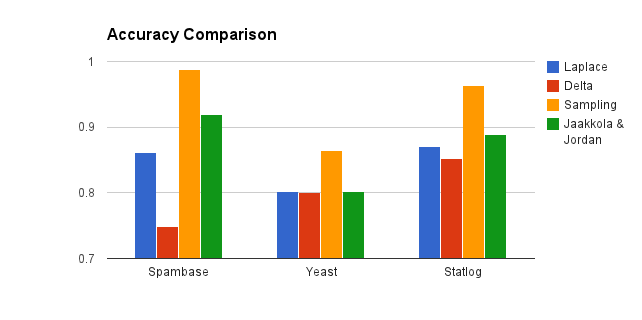
\includegraphics[height=7.0cm]{results/accuracy_comp.png}
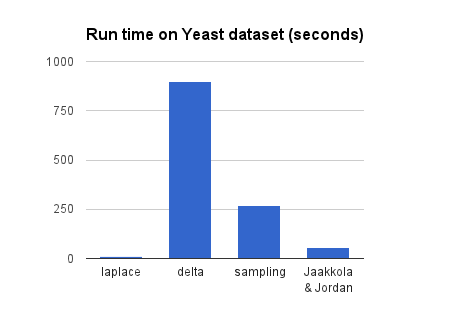
\includegraphics[height=8.0cm]{results/speed_comp.png}

\caption{\small Experiment results; {\bf Top:} Classification accuracy of all algorithms on
four datasets. {\bf Bottom:} Runtime for each algorithm on Yeast dataset. }
\label{fig:results}
\end{figure}

\subsubsection{MCMC based converging chains}
Our Kolmogorov Smirnove based Gibbs sampling strategy that we described in
section~\ref{sec:MCMCmethod} consistently to same set of parameters.
Figure~\ref{fig:MCMCconverge} is a plot of the iterations of the two
independent Markov chains for estimation on the spambase dataset. 
The X-axix of the figure represents the number of
iteration in sampling and Y-axis is the loglikelihood of the regression model.
As we can see both the chains converge to the same log-likelihood value and the
chains seem to be stable after convergence. Compare this to the markov chain
produce via uniform distribution based sampling methos in
figure~\ref{fig:uniformSamplerChain}. the chain in this case is not stable and
keeps oscillating between different log-likelihood states. 
 

\begin{figure}[hbt]
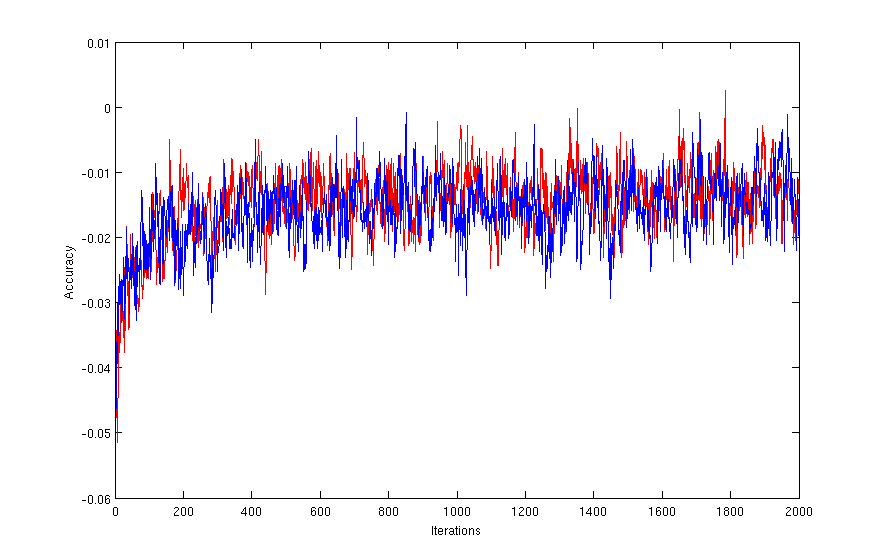
\includegraphics[width=1\textwidth]{results/KSsampleChain.png}
\caption{Two Markov chains (red and blue) converge on the same set of
parameters on the spambase dataset. The
X-axis is the number of iterations and Y-axis is the loglikelihood.}
\label{fig:MCMCconverge}
\end{figure}
